\section{Datenmodellierung}
    \subsection{ER-Modell}
        \includegraphics[page=16,trim=20 120 20 140,clip=true,width=0.5\textwidth]{images/datenmodellierung.pdf}
    \subsection{UML-Modell}
        \includegraphics[page=29,trim=20 30 20 85,clip=true,width=0.5\textwidth]{images/datenmodellierung.pdf}
    \subsection{Relationales Modell}
        \begin{description}
            \item[Entitität] Individuelles Element (Objekt) des betrachteten Systems
            \item[Relation] beschreibt eine Entitätsmenge
            \item[Tupel] repräsentiert eine Entität
        \end{description}
        \includegraphics[page=42,trim=10 30 0 84,clip=true,width=0.5\textwidth]{images/datenmodellierung.pdf}
    \subsubsection{Schlüssel}
    \begin{description}
        \item[Schlüssel] Attribute oder eine Kombination von Attributen, die ein Tupel eindeutig identifizieren.
        \item[Primärschlüssel] Der aus den möglichen Schlüsseln (= Schlüsselkandidaten) ausgewählte identifizierende Schlüssel. Wird für Fremdschlüsselbeziehungen verwendet.
        \item[Schlüsselkandidat] Attribut oder Kombination davon, das/die ein Tupel identifiziert.
        \item[Surrogatschlüssel] Künstlicher Schlüssel. Wird häufig eingeführt, wenn keiner der Schlüsselkandidaten obige Eigenschaften erfüllt.
    \end{description}
    \subsection{Relationale Schreibweise}
        \subsubsection{Tabellen}
            \begin{lstlisting}
TableName (
    Attr1 [Type] [PK] [NOT NULL|NULL] [UNIQUE] [REFERENCES TabName(Attr)],
    ...,
    
    [PRIMARY KEY CONSTRAINT(Attr1, Attr2, ...)]
)
            \end{lstlisting}
            \subsubsection{Attribut-Datentypen}
                \begin{itemize}
                  \item NUMBER, INT, INTEGER, DECIMAL[(10,2)]
                  \item TEXT, STRING, VARCHAR
                  \item TEXT(3), CHAR(3)
                  \item DATE, TIME, DATETIME
                  \item BOOLEAN
                  \item ENUM, ENUM(ROT,GELB), DOMAIN
                \end{itemize}
            \subsubsection{UML in relationales Modell}
                \paragraph{Abbildung von Klassen und Attributen}
                    \begin{itemize}
                        \item pro Klasse eine Tabelle
                        \item 1. Normalform, optionale Attibute mittels NULL
                        \item mindestens einen Primärschüssel
                    \end{itemize}
                \paragraph{Abbildung von Assoziationen und Aggregationen}
                \paragraph{Abbildung von Generalisierungen}